\documentclass{beamer}
\usepackage[utf8x]{inputenc}
%\usepackage{default}
\usepackage{verbatim}
\usepackage{graphicx}

\title{Combining Roborescue and XABSL}
\subtitle{Midterm Presentation}
\author{Maarten de Waard}
\institute{UvA}
\usetheme{Berkeley}
\newcommand{\slide}[2]
{
\begin{frame}
\frametitle{#1} 

#2

\end{frame}
}

\begin{document}
{
\usebackgroundtemplate{
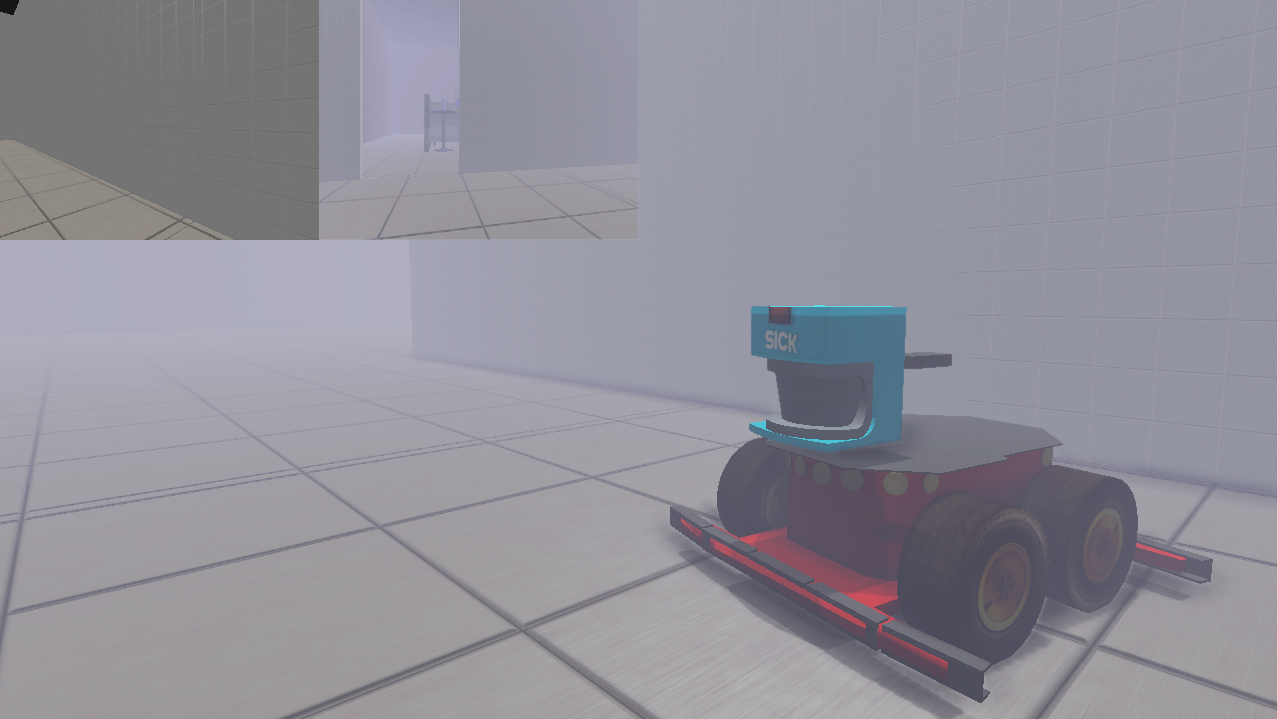
\includegraphics[width=\paperwidth, height=\paperheight]{interface}
}
\begin{frame}
\titlepage
\end{frame}
}

\section{Recap}
\slide{Recap}
{
    To freshen your memories, a short summary of my research and my goal:
    \begin{itemize}
        \item UvA Rescue - The UvA's virtual rescue operation
        \item XABSL - eXtended Agent Behavior Specification Language
        \item The combination - A thriving combination of UvA's Rescue research and Germany's winning robotic soccer team.
    \end{itemize}
}

\section{Challenges}
\subsection{Roborescue}
\slide{Roborescue}
{
    Problems with the system
    \begin{itemize}
        \item No Linux compatibility
        \item No user base (only Arnoud Visser uses it)
        \item Very little documentation
    \end{itemize}
    This causes problem solving to take more time than usual.
}
\subsection{VB and C++}
\slide{Visual Basic and C++}
{
    I have encountered some problems with these two languages:

    \begin{itemize}
    \item Both new languages
    \item I am new to the programming environment 
    \item Interfacing both using DLL's
    \end{itemize}
}
\subsection{XABSL}
\slide{XABSL}
{
    XABSL (eXtended Agent Behavior Specification Language) is the language I will use to 
    specify behaviors. It has a few down sides:
    \begin{itemize}
        \item Very small user base
        \item Very concise documentation
        \item Have to find out a lot myself
    \end{itemize}
}
\section{Current Status}
\slide{Current Status}
{
    So what is done, and what is yet to be done?\\
    Done:
    \begin{itemize}
        \item Installing entire framework
        \item Getting most of the framework (or at least enough) working
        \item Creating a C++ DLL, accessible from Visual Basic
        \item Creating a small XABSL hierarchy
    \end{itemize}
    To do:
    \begin{itemize}
        \item Combining XABSL with the current code
        \item Making a (good) Autonomous Exploration algorithm in XABSL
    \end{itemize}
}
\section{}
\slide{Questions}
{}



\end{document}
